\chapter{Макет интерфейса приложения}

Перед разработкой приложения был составлен макет интерфейса. На нем отражены следующие составляющие сайта:
\begin{itemize}
	\item элементы приложения, их вид и расположение;
	\item вид приложения при разных разрешениях экрана;
	\item цветовое решение;
	\item графические элементы;
	\item гарнитуры и шрифт текстов.
\end{itemize}

\begin{figure}[h!]
	\begin{subfigure}[l]{0.45\textwidth}
		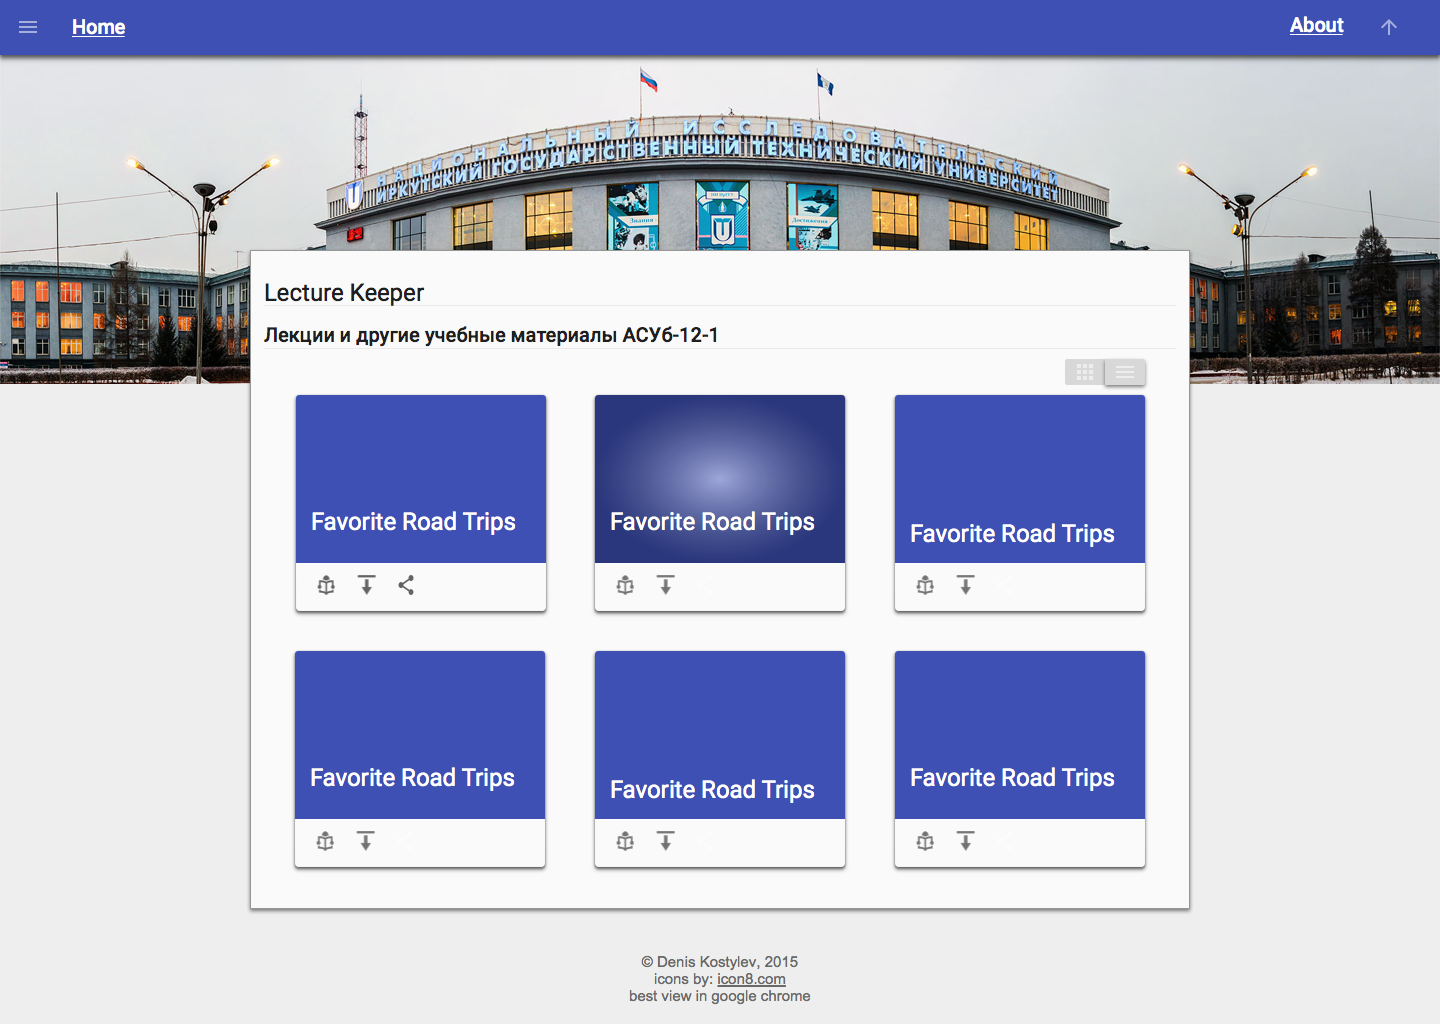
\includegraphics[width=\textwidth]{pics/sketches/main_card.png}
		\caption{Дисциплины в виде карточек}
	\end{subfigure}
	\quad
	\begin{subfigure}[r]{0.45\textwidth}
		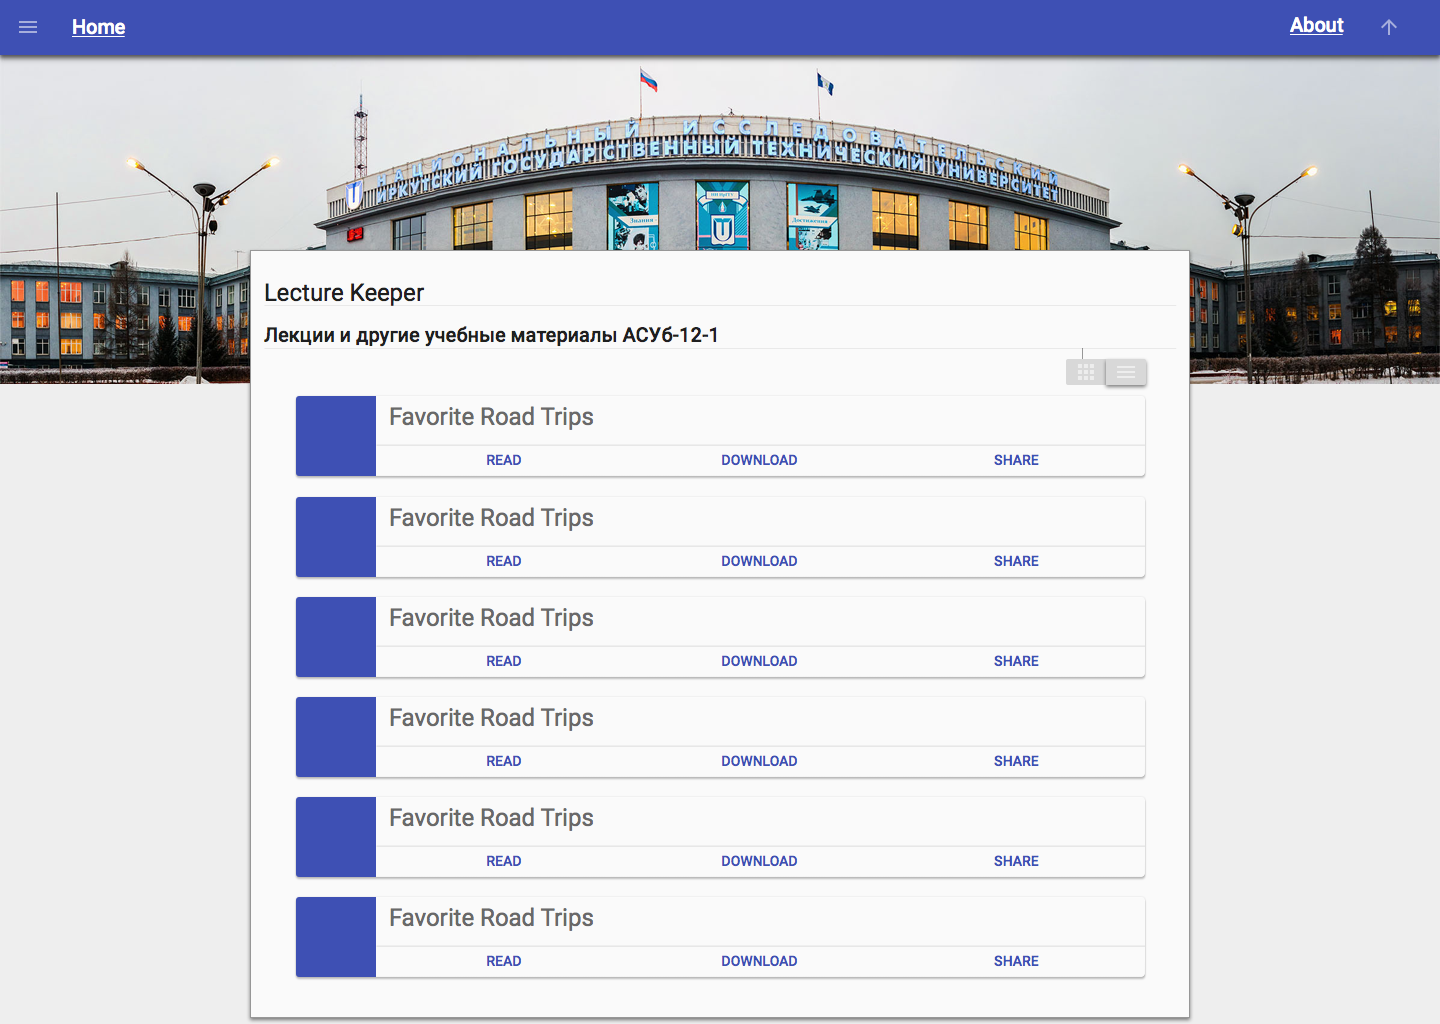
\includegraphics[width=\textwidth]{pics/sketches/main_list.png}
		\caption{Дисциплины в виде списка}
	\end{subfigure}
	\caption{Главная страница приложения}
\end{figure}

%\begin{figure}
%	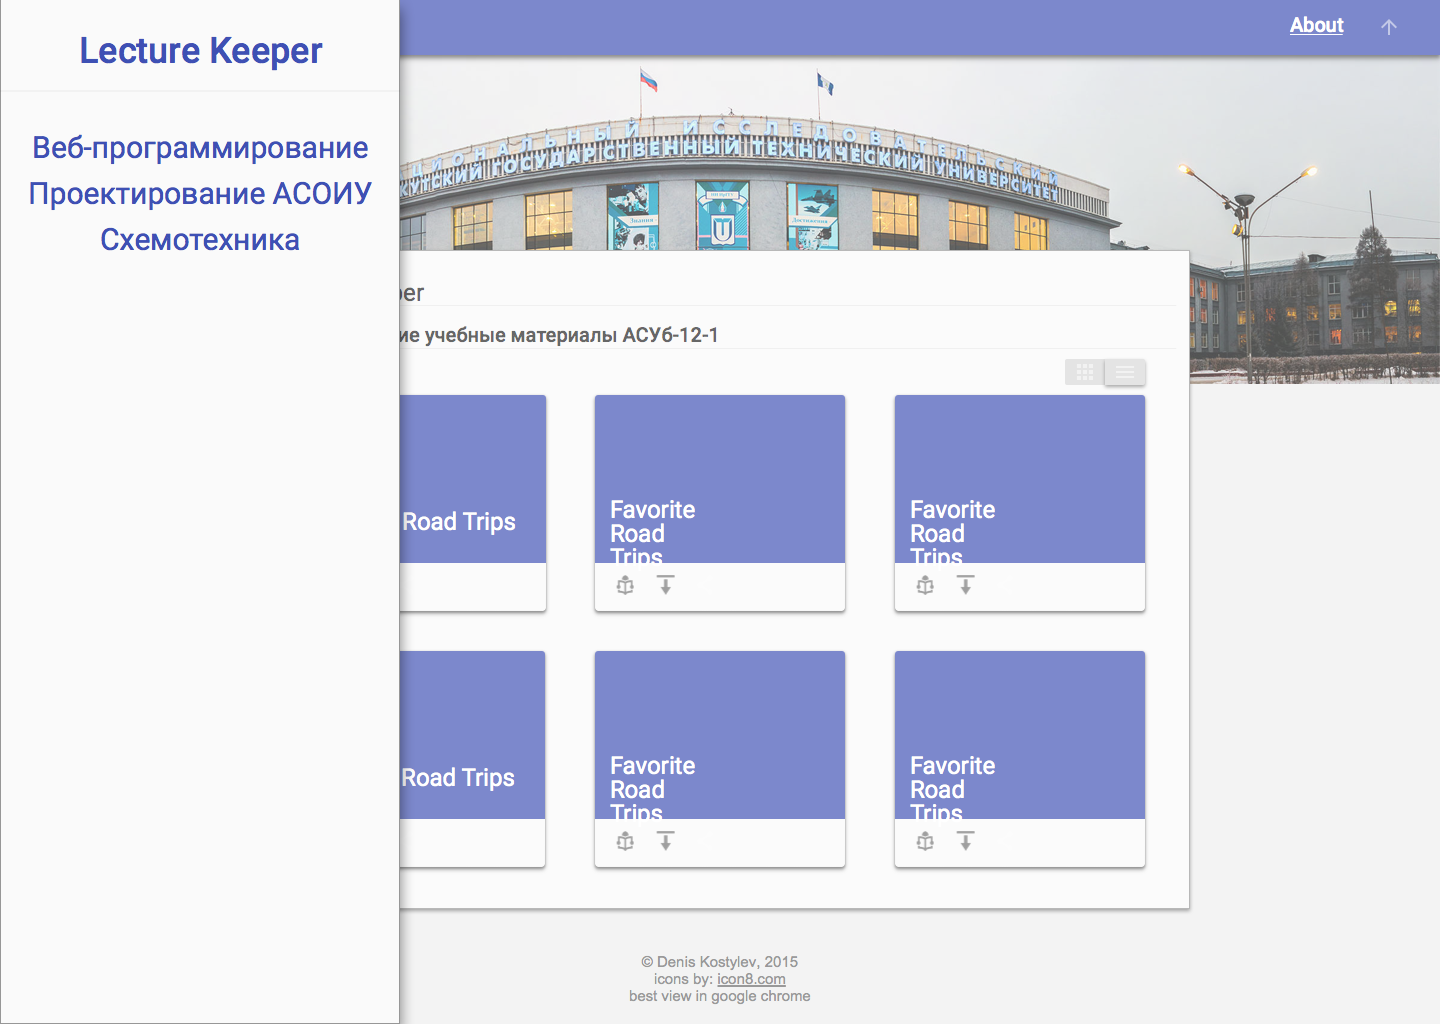
\includegraphics{/sketches/menu.png}
%	\caption{Меню приложения}
%\end{figure}
%
%\begin{figure}
%	\begin{subfigure}
%		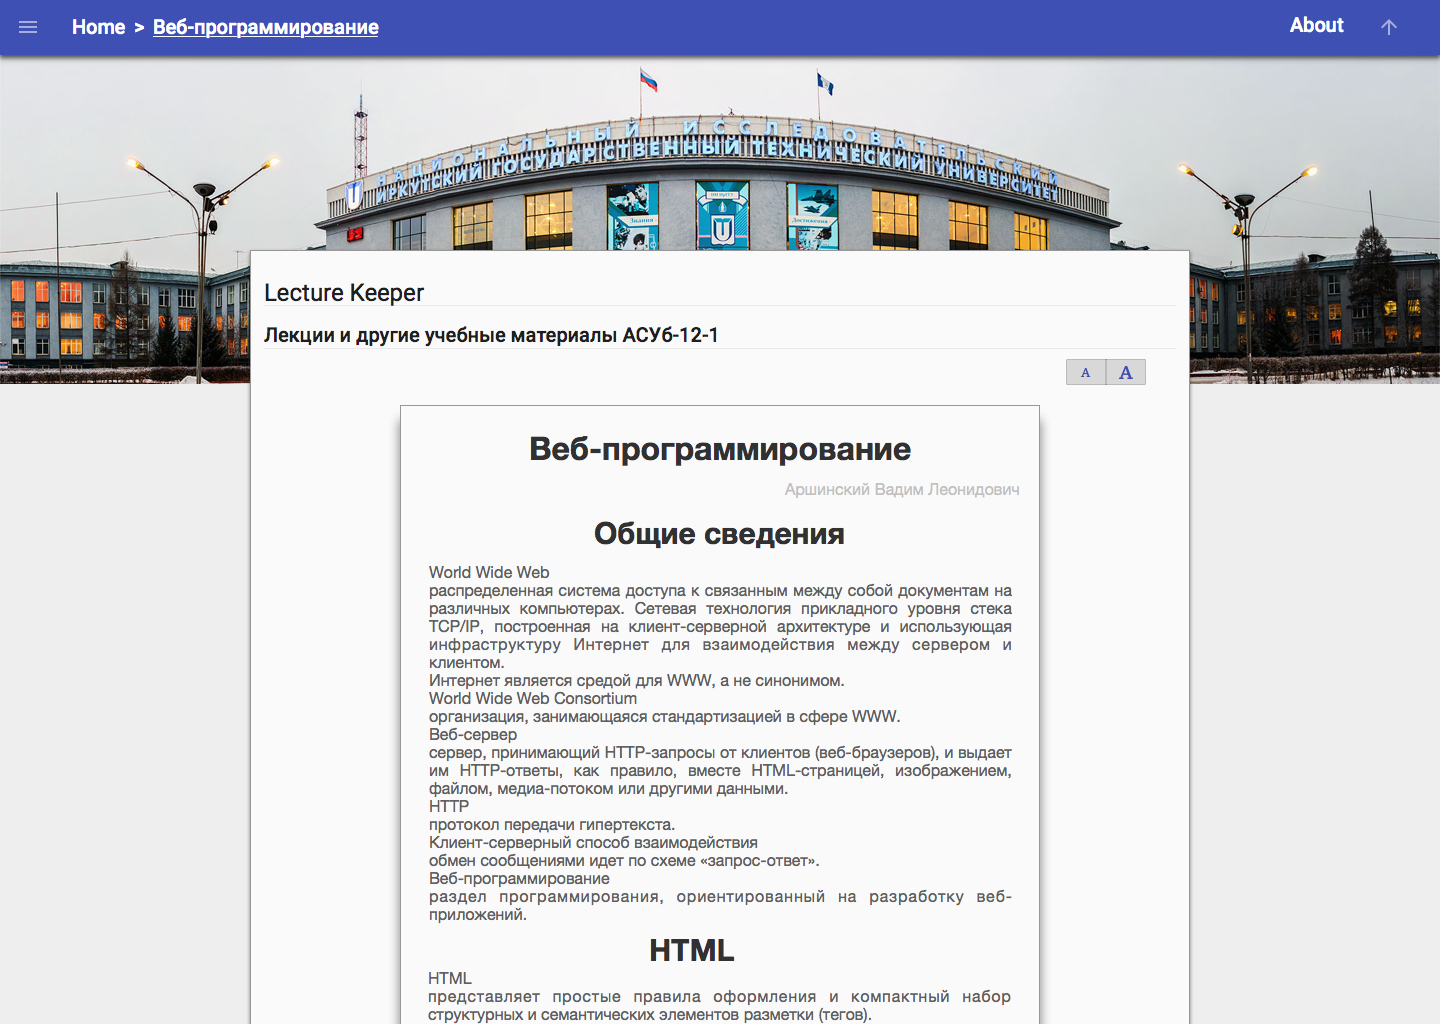
\includegraphics{/sketches/lecture.png}
%		\caption{Страница лекции}
%	\end{subfigure}
%	\begin{subfigure}
%		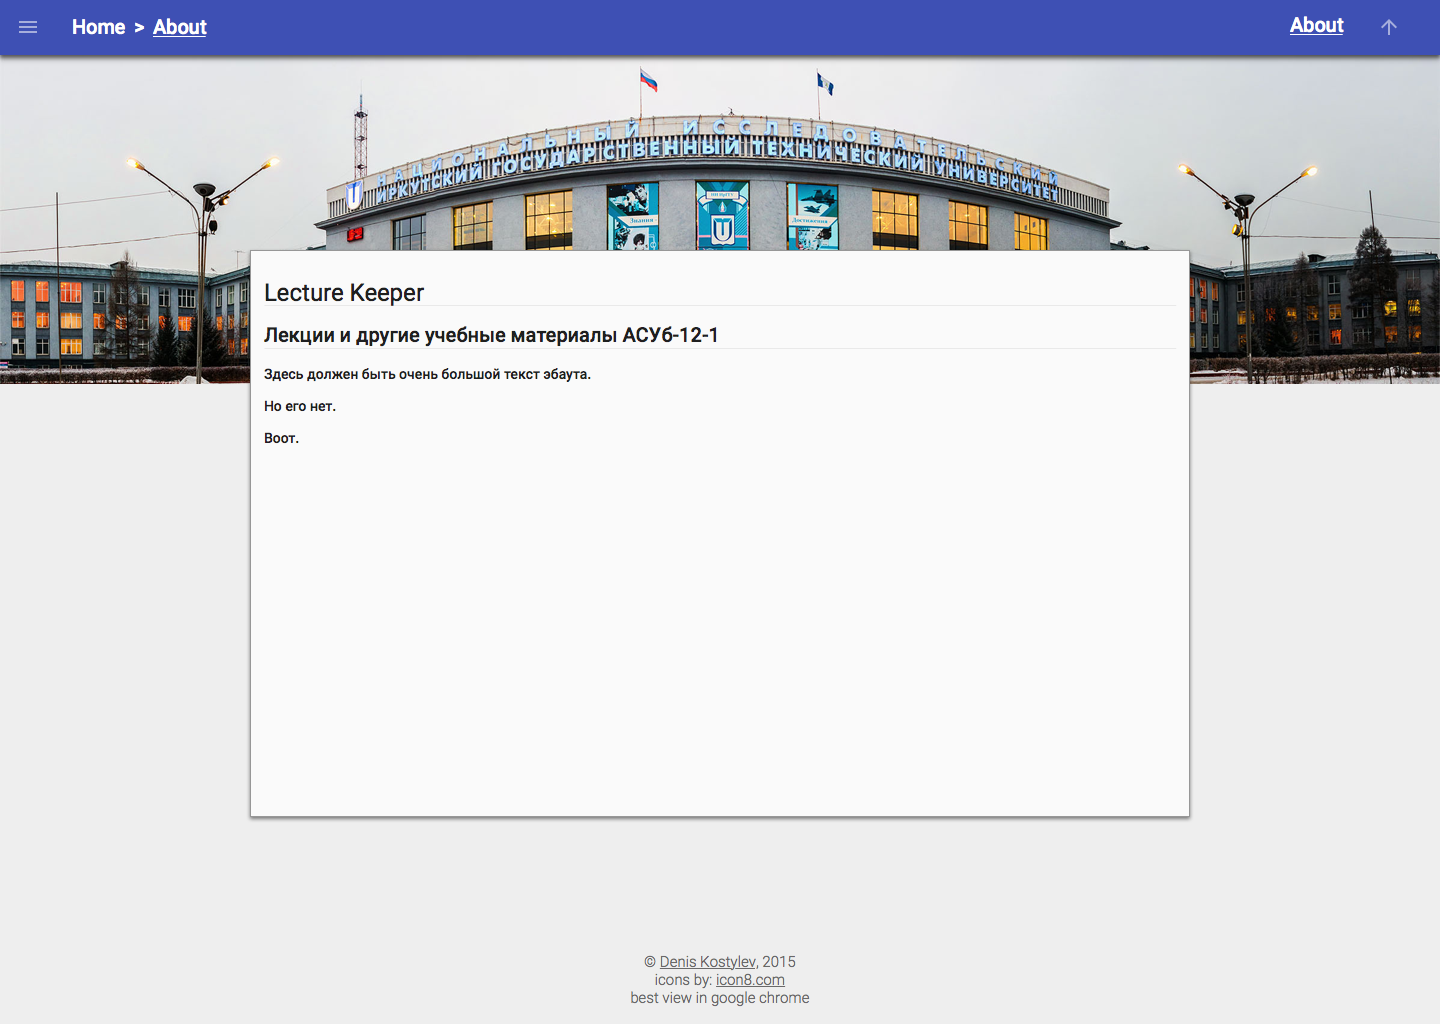
\includegraphics{/sketches/about.png}
%		\caption{Страница "О сайте"}
%	\end{subfigure}
%	\caption{Страницы с содержимым}
%\end{figure}
%
%\begin{figure}
%	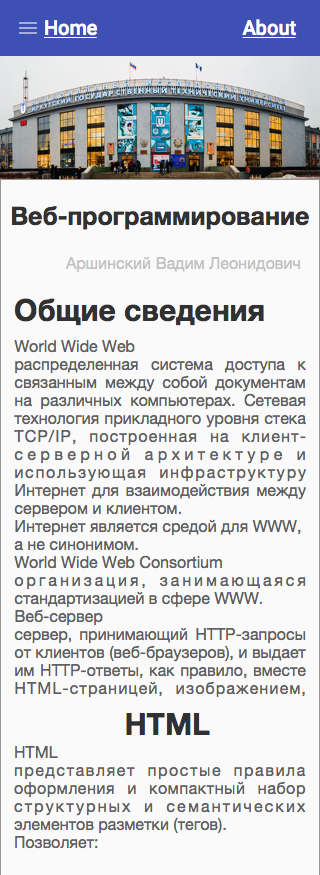
\includegraphics{/sketches/mobile.png}
%	\caption{Главная страница для мобильных устройств}
%%%\end{figure}